\documentclass[10pt]{beamer}

\usetheme[progressbar=frametitle,block=fill,background=light]{metropolis}
%\usefonttheme{serif}

\usepackage{appendixnumberbeamer}

\usepackage{booktabs}
\usepackage[scale=2]{ccicons}
\usepackage{nicefrac}

\usepackage{pgfplots}
\usepgfplotslibrary{dateplot}
\usepackage{pgfplotsthemetol}

\usepackage{xspace}
\newcommand{\themename}{\textbf{\textsc{metropolis}}\xspace}

\title{Group theory, Topology and Spin-$1/2$ Particles}
\subtitle{From Dirac's belt to fermions}
% \date{\today}
\date{}
\author{Louan Mol}
\institute{Unversité Libre de Bruxelles\\[2cm]{\small Brussels Summer School of Mathematics 2022}}
% \titlegraphic{\hfill\includegraphics[height=1.5cm]{logo.pdf}}

\begin{document}

\maketitle

\begin{frame}{Table of contents}
  \setbeamertemplate{section in toc}[sections numbered]
  \tableofcontents%[hideallsubsections]
\end{frame}

\section[Intro]{Dirac's belt trick and rotations}

    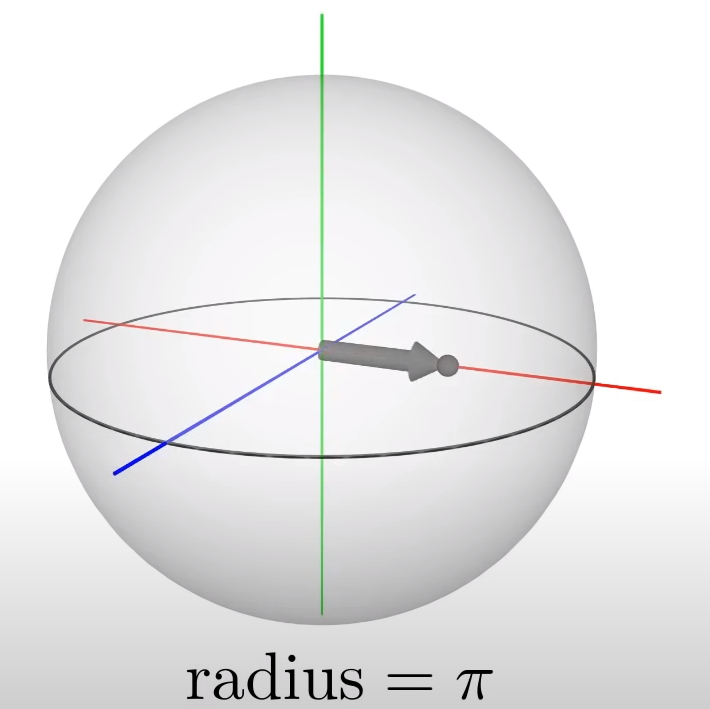
\includegraphics[scale=0.1]{Pictures/SO3sphere.png}

    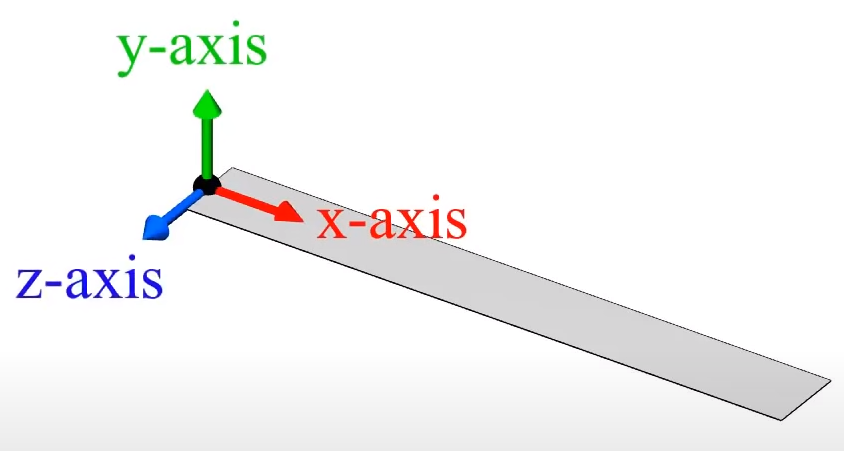
\includegraphics[scale=0.1]{Pictures/beltaxis.png}

    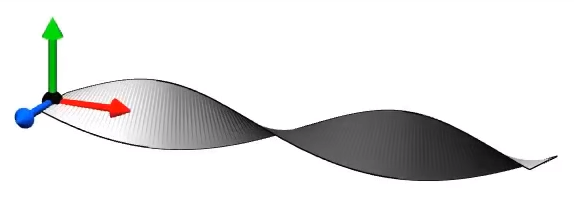
\includegraphics[scale=0.1]{Pictures/xaxisbelt.png}

    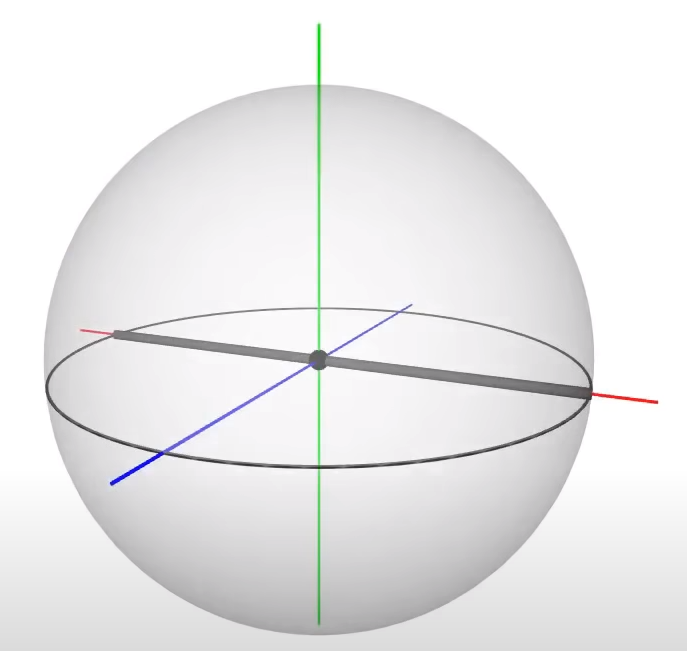
\includegraphics[scale=0.1]{Pictures/xaxissphere.png}

    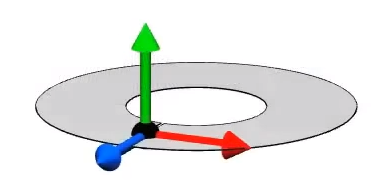
\includegraphics[scale=0.1]{Pictures/yaxisbelt.png}

    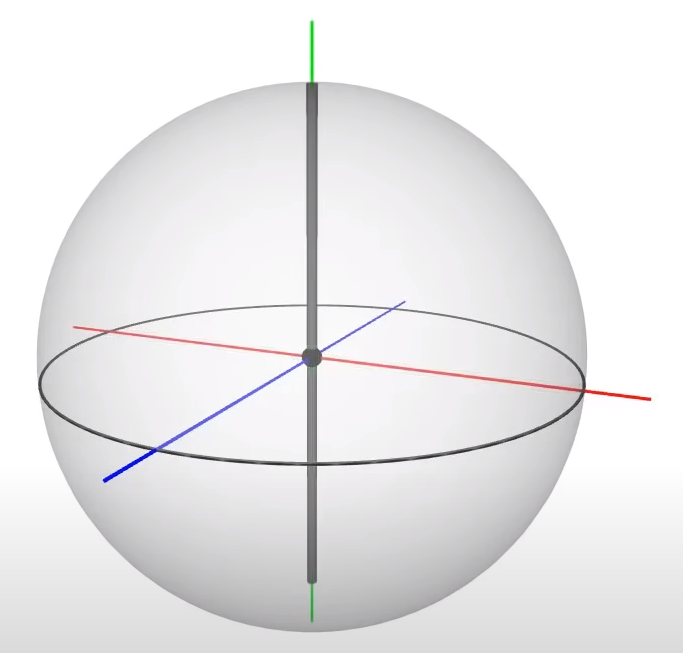
\includegraphics[scale=0.1]{Pictures/yaxissphere.png}

    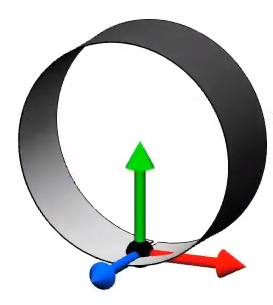
\includegraphics[scale=0.1]{Pictures/zaxisbelt.png}

    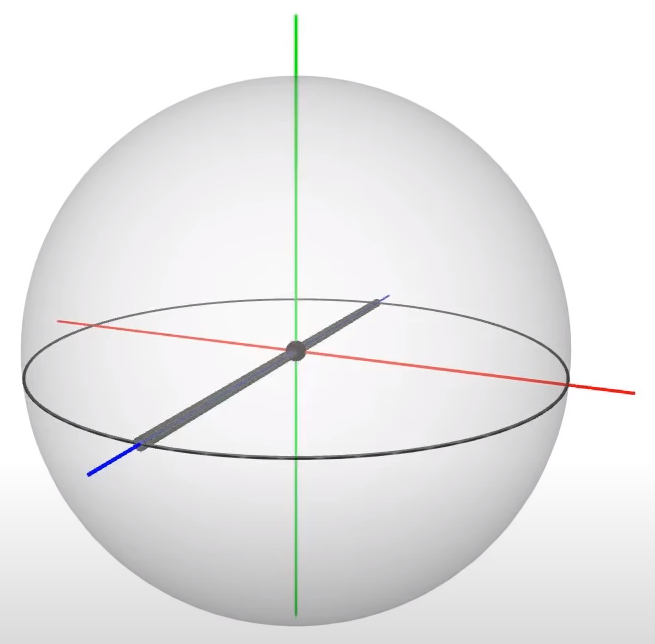
\includegraphics[scale=0.1]{Pictures/zaxissphere.png}

    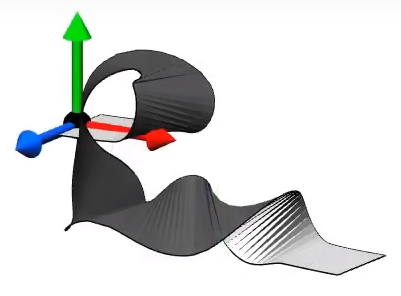
\includegraphics[scale=0.1]{Pictures/randomrotbelt.png}

    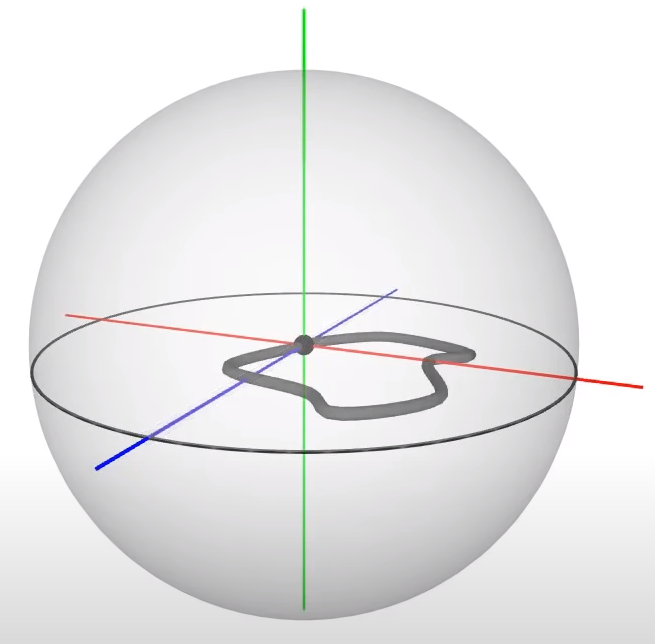
\includegraphics[scale=0.1]{Pictures/randomrotsphere.png}

    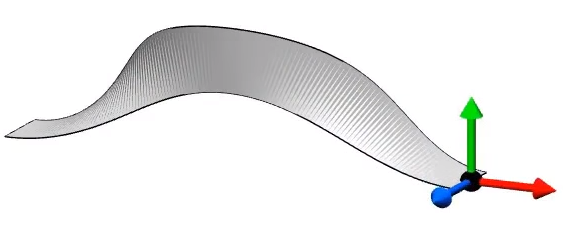
\includegraphics[scale=0.1]{Pictures/contractiblepathbelt.png}

    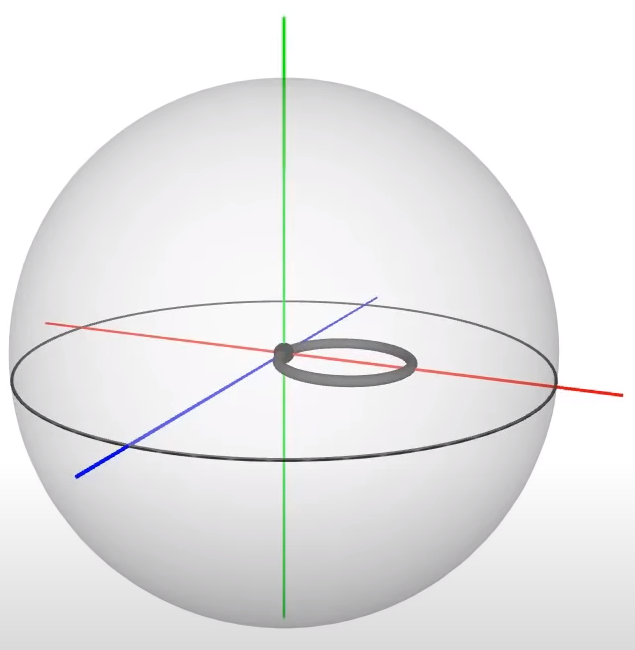
\includegraphics[scale=0.1]{Pictures/contractiblepathsphere.png}

    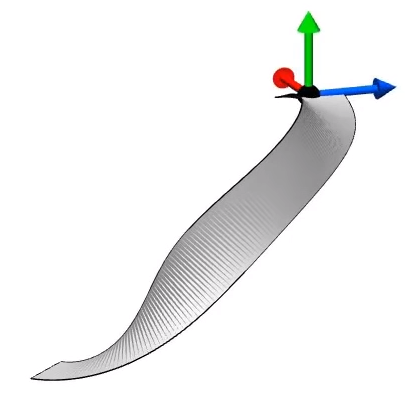
\includegraphics[scale=0.1]{Pictures/noncontractiblepathbelt.png}

    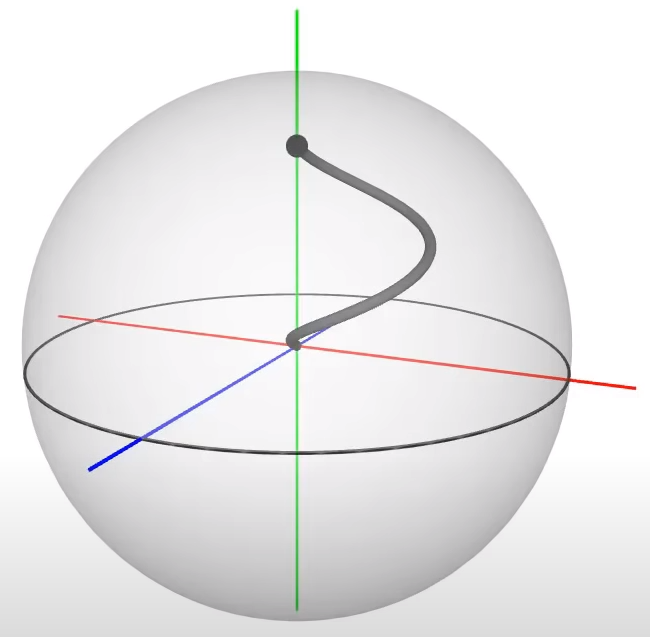
\includegraphics[scale=0.1]{Pictures/noncontractiblepathsphere.png}

    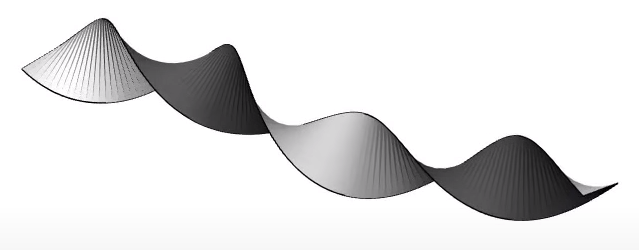
\includegraphics[scale=0.1]{Pictures/4pibelt.png}

    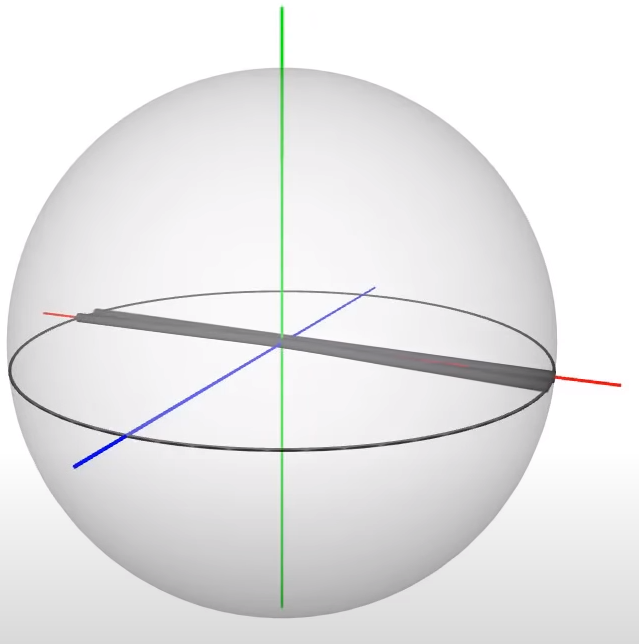
\includegraphics[scale=0.1]{Pictures/4pisphere1.png}

    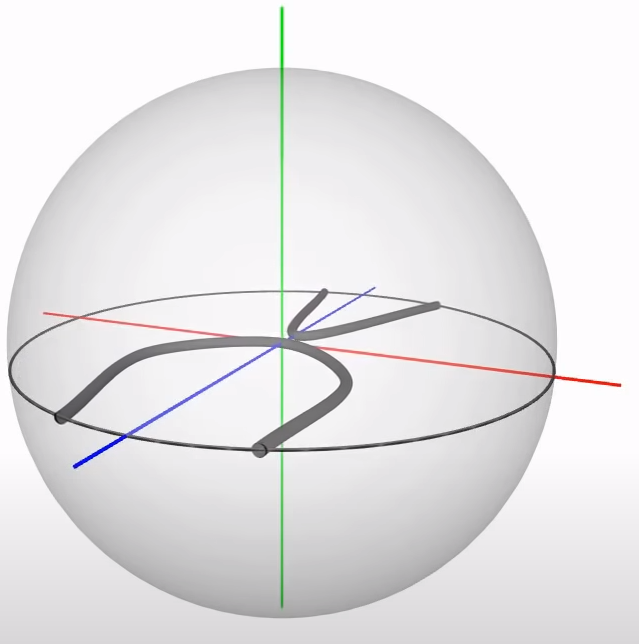
\includegraphics[scale=0.1]{Pictures/4pisphere2.png}

    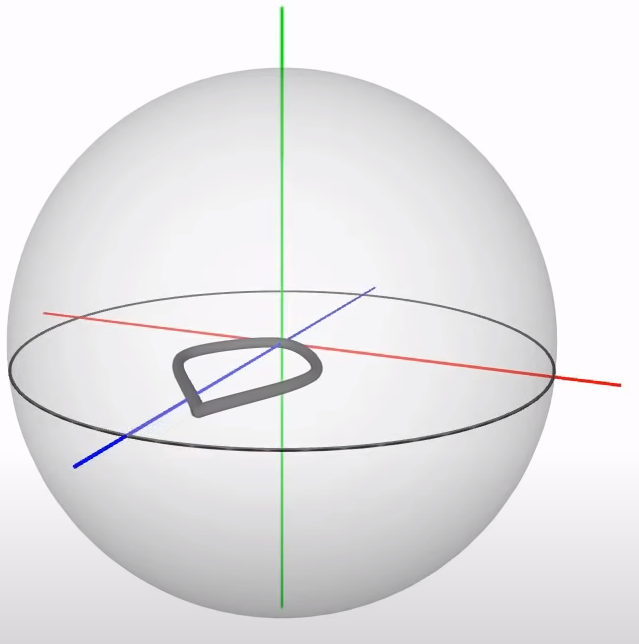
\includegraphics[scale=0.1]{Pictures/4pisphere3.png}

    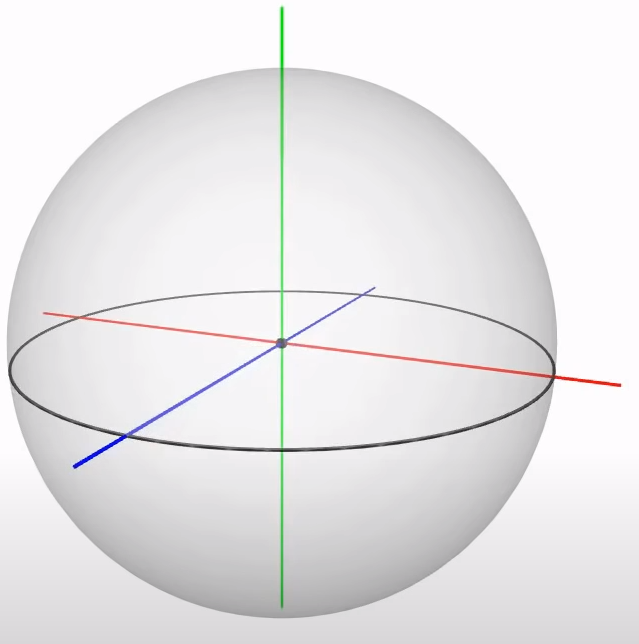
\includegraphics[scale=0.1]{Pictures/4pisphere4.png}

    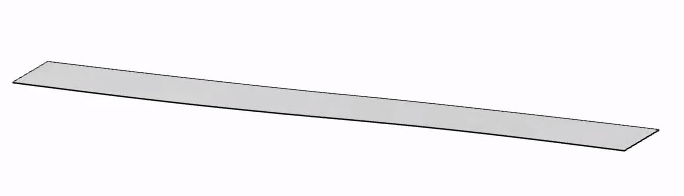
\includegraphics[scale=0.1]{Pictures/flatbelt.png}

\section{Section 2}

\section{Section 3}

\section{Section 4}

\section{Section 5}

\begin{frame}{Blocks}
    Three different block environments are pre-defined and may be styled with an
    optional background color.
  
    \begin{columns}[T,onlytextwidth]
        \column{0.5\textwidth}
          
            Some text.\\[2cm]
            aaaaa
    
        \column{0.5\textwidth}
    
          \begin{block}{Default}
            Block content.
          \end{block}
    
          \begin{alertblock}{Alert}
            Block content.
          \end{alertblock}
    
          \begin{exampleblock}{Example}
            Block content.
          \end{exampleblock}
    
      \end{columns}

  \end{frame}

\appendix

\begin{frame}[fragile]{Backup slides}
  Sometimes, it is useful to add slides at the end of your presentation to
  refer to during audience questions.

  The best way to do this is to include the \verb|appendixnumberbeamer|
  package in your preamble and call \verb|\appendix| before your backup slides.

  \themename will automatically turn off slide numbering and progress bars for
  slides in the appendix.  \cite{ConcreteMath}
\end{frame}

\begin{frame}[allowframebreaks]{References}

  \bibliography{bibliography}
  \bibliographystyle{abbrv}

\end{frame}

\end{document}
